\section{Pilot Experiments}\label{sec:prelim}
In this section, we explain our preliminary experiments which led to the design of our intent generation model.
The goal of the pilot experiments presented in this section is to determine if a specific architecture could benefit our task, so we consider simple variants of major architecture families which could fit our goal. Also, the architectures are not trained to their maximum, and even if the results are not conclusive, it does not mean that an architecture in itself has no potential. However it hints a lower potential improvement of the performance for our task.
We consider 3 families of architectures for the task, each requiring some preliminary assumption on the size of the data:
\begin{itemize}
    \item the VAE architecture requires to have a fixed input and output size, so all the dimensions ($|O|$, $|A|$, and $|I|$) must be defined when creating a model; it is presented in \cref{sec:prelim-vae};
    \item the CNN architecture only requires to have a fixed $|I|$; it is presented in \cref{sec:prelim-cnn};
    \item the LSTM architectures only require to have a fixed $|A|$; it is presented in \cref{sec:prelim-lstm}.
\end{itemize}
We explain those limitations in the following subsections.
In each case, a model will be able to handle smaller inputs and outputs, but nothing larger than the values given creating the model.


%The results presented here all follow the same structure: first row is the output of the model (the prediction), and second row is the expected output. each column correspond to a sample of the data (one context/lattice pair).

\subsection{Variational Auto-Encoder Architecture}\label{sec:prelim-vae}
The VAE architecture is structurally the simplest of all the tested architecture.
It takes as an input a flattened FC at once and the output is reshaped into an intent matrix.
The encoder and the decoder are two MLPs. A block diagram of the architecture is shown in \cref{fig:prelim-vae-block}.

Using MLPs directly forces the input and output to always have the same size.
In this setup, we need to define $|O|$, $|A|$, and $|I|$ when we create the model.
Typically, those should be the maximal values in dataset of $|O|$, $|A|$, and $|I|$.
Using padding will allow us to process samples with smaller dimensions, but the model will be unable to process larger samples without loosing information.

This architecture is very simple and performs well, as shown in \cref{fig:prelim-vae}.
Indeed, the VAE seems to produce the expected shape and spread of the attributes across the contexts: few attributes for the intents close to $\top$, and more and more attributes until we reach $\bot$.
However, the fixed input and output size is a major drawback of this approach.

\subsection{Convolutional Neural Network Architecture}\label{sec:prelim-cnn}
The CNN architecture offers flexibility in the size of the input and output.
However, the size of the output of a CNN is proportional to the size of its input (due to the convolution principle).
In our case, it would mean that the number of predicted concepts would be directly proportional to the number of objects, which seems quite strange especially since that the theoretical upper bounds (see \cref{sec:boa-metric}) make the number of concept an exponential of the size of the FC.
With a standard CNN, the relation between the number of input objects and the number of output intents would have to be defined when designing the architecture, which seems unreasonable due to the explosive nature of the number of potential concepts.
 
To avoid the issue described above, we use one output \textit{channels} of the CNN for each concept, leading to the architecture schematized in \cref{fig:prelim-cnn-block}.
Consequently, we do not have a relation between the number of objects and the number of concepts nor any constraint on the number of objects, even if we still require the maximum $|I|$.
Interestingly, there is a full ``view'' on the data dedicated to each concept because each channel serves as a parallel and independent ``view'' on the FC.
The tested CNN requires a lot of parameters to compensate for removing the constraint on the object number. This large amount of parameters and its internal structure gives it a greater learning capability than the VAE. 

As shown in \cref{fig:prelim-cnn}, the shape of the output is close to the expected one and the spread of the attributes matches the expected output, similarly to the results of the VAE.
The results of the CNN look a little more random than the ones of the VAE, even if the ``texture'' (the sharpness of the result) of the predictions by the CNN is closer tho the expected output than the one produced by the VAE.
This approach seem to perform comparably to VAE, but with only a constraint on $|I|$.

\begin{figure}
    \centering
    \subcaptionbox{VAE\label{fig:prelim-vae-block}}{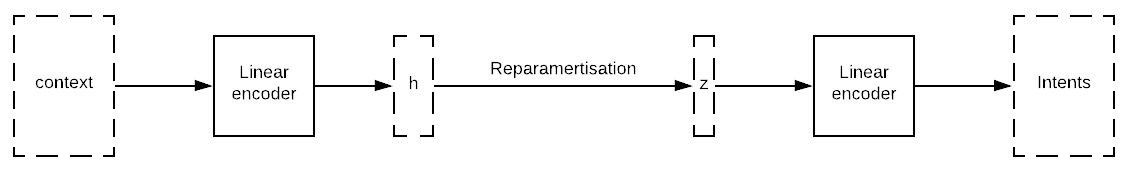
\includegraphics[width = .9\textwidth, height = 4cm, keepaspectratio]{Figures/Ch3/vae_block.png}}
    \subcaptionbox{CNN\label{fig:prelim-cnn-block}}{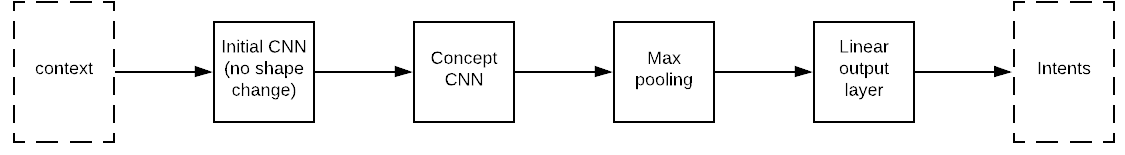
\includegraphics[width = .9\textwidth, height = 4cm, keepaspectratio]{Figures/Ch3/cnn_block.png}}
    \caption{Block diagrams of the VAE and CNN architectures.}
\end{figure}

\begin{figure}
    \centering
    \subcaptionbox{VAE\label{fig:prelim-vae}}{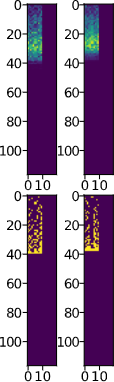
\includegraphics[width = .9\textwidth, height = 6cm, keepaspectratio]{Figures/Ch3/vae.png}}
    \subcaptionbox{CNN\label{fig:prelim-cnn}}{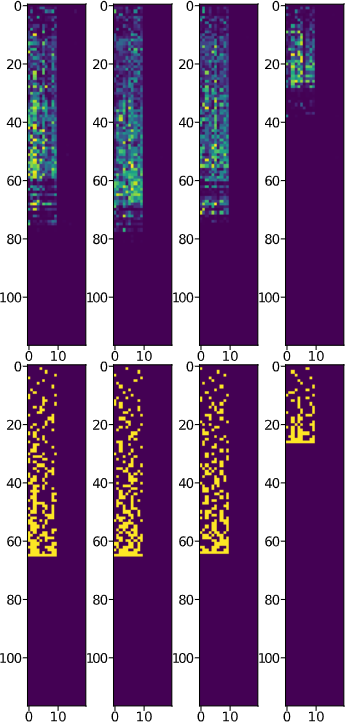
\includegraphics[width = .9\textwidth, height = 6cm, keepaspectratio]{Figures/Ch3/cnn.png}}
    \caption{Examples of results of the VAE and CNN architectures. In the images, a blue pixel corresponds to a $0$ and a yellow one to $1$. The first row correspond to the prediction by the model and the second row is the actual intent matrix. Each column correspond to a different sample in the same batch.}
\end{figure}

\subsection{Recurrent Neural Network Architecture and Attention Mechanisms} \label{sec:prelim-lstm}
\begin{figure}
    \centering
    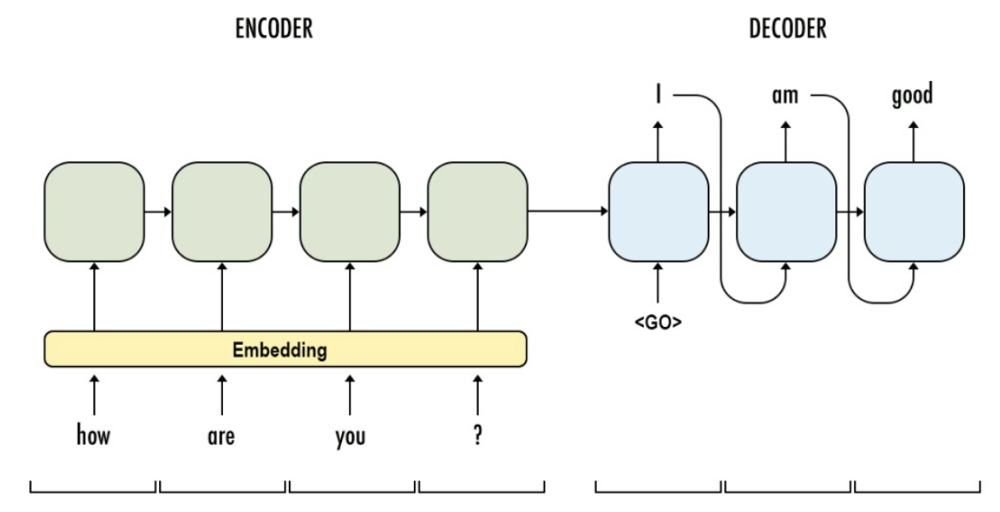
\includegraphics[width = .8\textwidth, height = .4\textwidth, keepaspectratio]{Figures/Ch3/seq2seq.png}
    \caption{Example of a sequence to sequence RNN, figure from~\cite{nlp:2018:aditya}.}
    \label{fig:seq2seq}
\end{figure}

We use LSTM as a sequence to sequence model (\textit{seq2seq}), a common way to use the RNN to produce an output which does not have the same size as the input, \eg, \cref{fig:seq2seq}. Indeed, in our case, the number of concepts is different from the number of objects.
We use the attribute dimension as the input and output size, and the object and concept dimension as the sequence dimension. Due to this, the model is constrained the maximum $|A|$.
We experiments with a few variants of attention mechanisms:
\begin{itemize}
    \item \textit{soft-attention}, which compute a summary of all the inputs with respect to the current output, and use this summary to improve the current output;
    \item \textit{self-attention}, which compute a summary of the previous outputs with respect to the current output, and use this summary to improve the current output;
    \item a variant for our case of self-attention: \textit{link-attention}, which compute the similarity of the previous outputs with respect to the current output, and this similarity (between 0 and 1) serves as a link prediction; more precisely, the similarity between previous output $i$ and current output $j$ represent the probability to have a link between concept $i$ and concept $j$.
\end{itemize}
We use a simple version of attention, with $\cdot$ the dot product, $q$ the \textit{query} (the current LSTM output in our case), $s$ the sequence. We first compute the attention weight for a value $v\in s$ as $w_{q, v} = q \cdot v$, and apply a softmax on all the weights. Because after the softmax the sum of the weights is 1, the attention context $a_{q,s} = \sum_{v\in s}{w_{q, v}}$ also corresponds to the weighted average of the input sequence.
The global structure of the recurrent architecture is presented in \cref{fig:lstm_block}, with the three attention mechanisms in different colors.
Because we want to check whether using a specific attention mechanism improves the output, we test 5 variants of the architecture listed bellow, and compare the results along the arrows on \cref{fig:rnn_variants}.

\begin{figure}
    \centering
    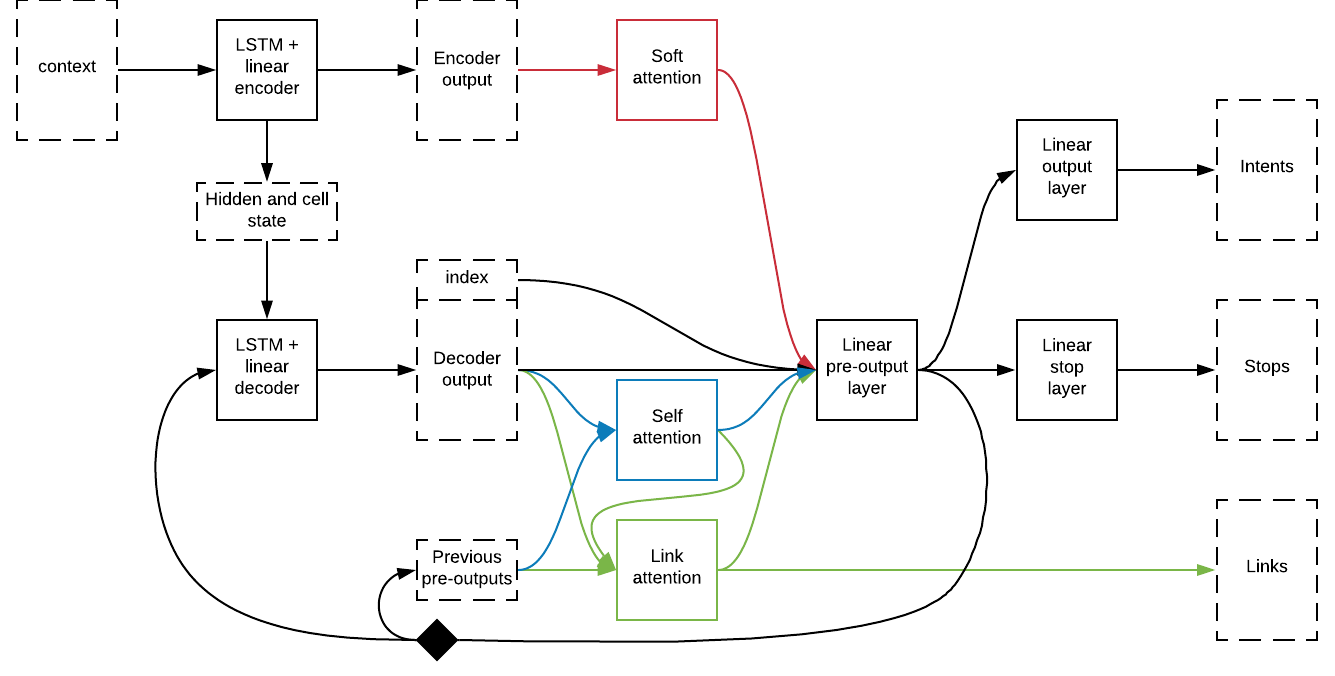
\includegraphics[width = .8\textwidth, height = .4\textwidth, keepaspectratio]{Figures/Ch3/lstm_block.png}
    \caption{Block diagram of the recurrent architectures.}
    \label{fig:lstm_block}
\end{figure}

The \textit{basic} model uses no attention, and takes the FC as a sequence of objects in input, and produces a sequence of intents in output.
Also, a second output is produced: the stop vector. It serves to determine when to stop generating intents during real-case usage.
In this specific implementation, the stop vector contains 1 if the corresponding row is a context intent, 0 if it is just padding.
%
The \textit{soft-attention} model extends the basic model with the soft-attention mechanism, which should improve the relevance of the output \textit{w.r.t.} the input because the model has a better access to the input information.
%
The \textit{self-attention} model extends the basic model with self-attention, which should improve the internal coherence of the output, as the model has a better access to the previously generated intents. We should obtain, \eg, a gradient from the empty set to the full set of attributes and a better prediction of the stop vector.
%
The two attention mechanisms are used in the \textit{bi-attention} model, so we can expect this model to bring the improvements of the self- and soft- attention together.
%
Finally, the \textit{tri-attention} model extends the bi-attention model with a link-attention as predicted above.
It generates an additional output: the links between the concepts, in other words the adjacency between the concepts. In our case we predict $\leq$, as we expect it to be easier to learn then $\prec$. Indeed, for $\leq$, a generic subset relation is enough, while for $\prec$ an additional step is required.

\begin{figure}
    \centering
    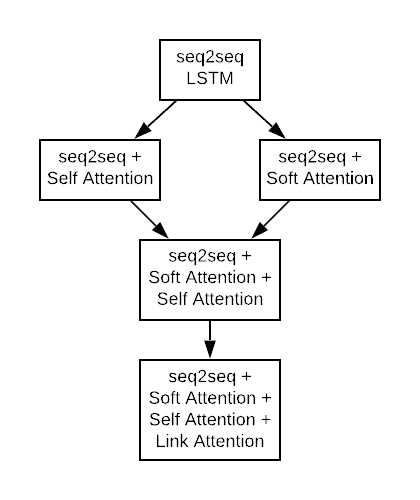
\includegraphics[width = .8\textwidth, height = .4\textwidth, keepaspectratio]{Figures/Ch3/rnn_attention.png}
    \caption{Hierarchy of the tested recurrent architecture variants}
    \label{fig:rnn_variants}
\end{figure}

The basic model performs quite bad (see \cref{fig:rnn}), which is to be expected given the complexity of the data and the relative simplicity of the model. All the produced intents look similar, and are most likely a sort of average of all the intents in the training set, and the stop vector is not at all predicted. Not much impact of the input can be seen, which is to be expected: it is too ``far'' from the output for a simple LSTM to handle. 
%
The soft-attention improves the model in a noticeable, and expected, manner: the output now has the same number of attributes as the input (see \cref{fig:soft}).
%
The self-attention also fulfills our expectations: the output has a nicer gradient (compared to the basic model) and the stop vector begins to be predicted correctly.
An unexpected improvement is that the output now also has the same number of attributes as the input.
In \cref{fig:self} display those improvement, and one can also notice an interesting ``bar'' around the end of the prediction, which seem to correspond to $\bot$, hinting a large potential improvement of the stop prediction in case of further training.
%
The bi-attention produces the expected results too: the output has the correct number of attributes, a the stop vector is closer to the expected one, and the length of the output matches quite well the expected one (as we can see on \cref{fig:bi}, with sample 2 being predicted slightly longer than sample 3, which matches the expected output).

However, the tri-attention produces both expected and unexpected effects. 
As expected, the links in  \cref{fig:tri2} look close to the expected output which hints that link attention is beneficial and can be used to predict the relations between concepts.
%
A first noteworthy point is that the performance of the model varies from good (see \cref{fig:tri2}) to bad, depending on the random initialization. We suppose that training all 3 outputs (intents, stops and links) at the same time from scratch, is too much for the model, and that training one aspect alone before introducing the others could avoid this type of issue. The negative impact of those training issues on the performance cannot be neglected.
%
The second interesting point is that the stops in \cref{fig:tri2} are close to the expected output, and the intents and links are clearly impacted by the stops.
%
Finally, we don't have too much of a degradation of the performance from the bi-attention model despite the training difficulties, even if the number of attributes is less well-predicted. 

\begin{figure}
    \centering
    \subcaptionbox{Extract of a result with the the recurrent model.
    \label{fig:rnn}}{
    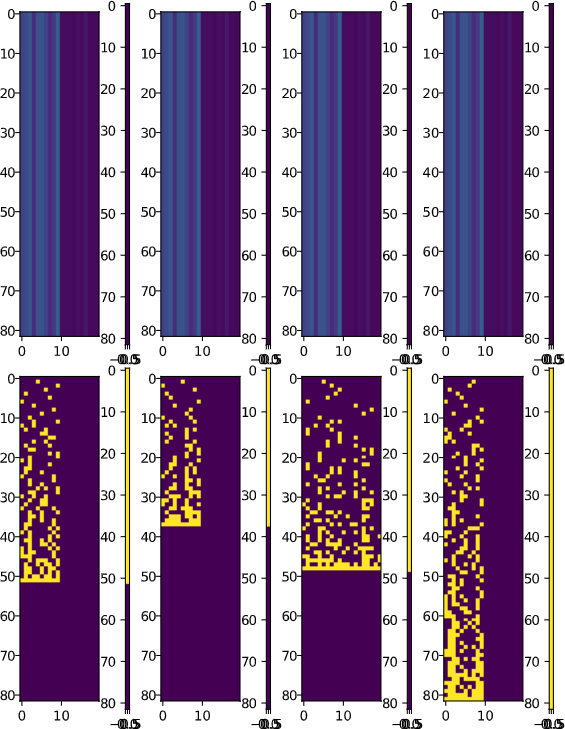
\includegraphics[width = .8\textwidth, height = .35\textwidth, keepaspectratio]{Figures/Ch3/rnn.png}}\hspace{2em}
    \subcaptionbox{Extract of a result with the soft-attention model.
    \label{fig:soft}}{
    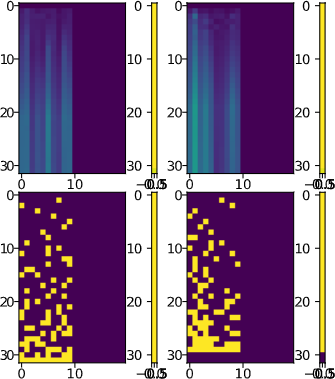
\includegraphics[width = .8\textwidth, height = .35\textwidth, keepaspectratio]{Figures/Ch3/soft.png}}\hspace{2em}
    \subcaptionbox{Extract of a result with the self-attention model.
    \label{fig:self}}{
    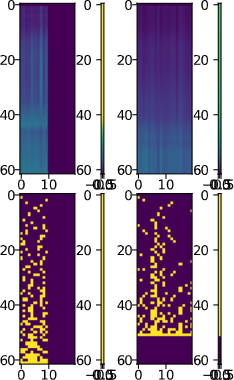
\includegraphics[width = .8\textwidth, height = .35\textwidth, keepaspectratio]{Figures/Ch3/self.png}}
    
    \subcaptionbox{Extract of a result with the bi-attention model.
    \label{fig:bi}}{
    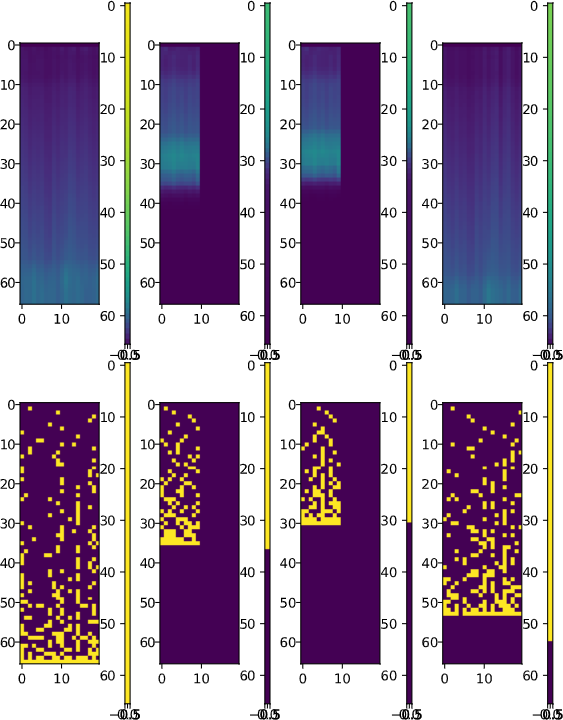
\includegraphics[width = .8\textwidth, height = .35\textwidth, keepaspectratio]{Figures/Ch3/bi.png}}\hspace{2em}
    \subcaptionbox{Extract of a result with the \nth{2} iteration of the tri-attention model.
    \label{fig:tri2}}{
    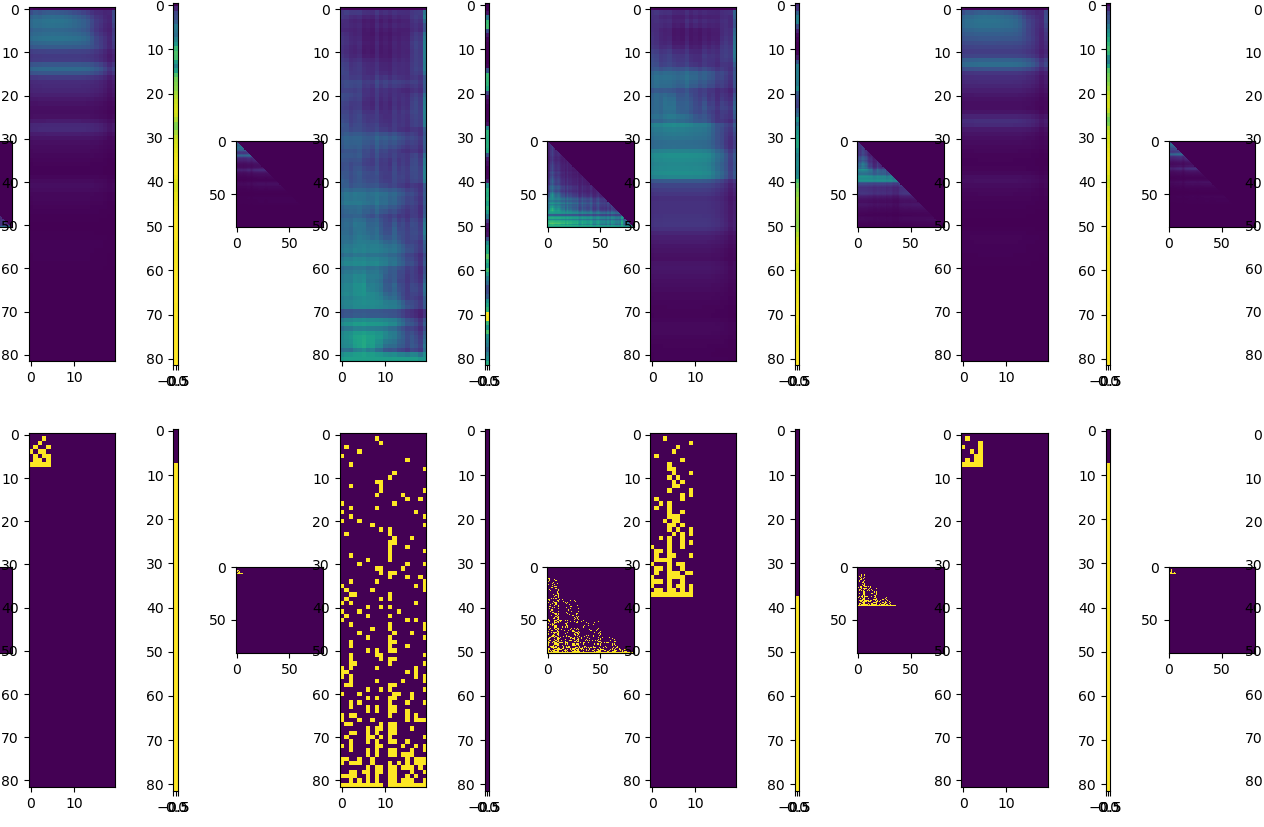
\includegraphics[width = .8\textwidth, height = .35\textwidth, keepaspectratio]{Figures/Ch3/tri2.png}}\hspace{2em}
    %\subcaptionbox{Extract of a result with the \nth{3} iteration of the tri-attention model.
    %\label{fig:tri3}}{
    %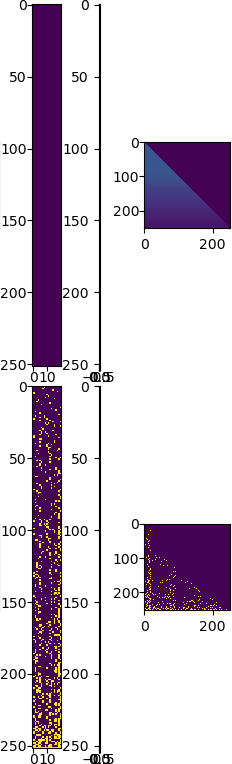
\includegraphics[width = .8\textwidth, height = .35\textwidth, keepaspectratio]{Figures/Ch3/tri3.png}}
    \caption{Extract of results on the test set with the various variants of the LSTM model. In the images, a blue pixel corresponds to a $0$ and a yellow one to $1$. The first row correspond to the prediction by the model and the second row is the actual intent matrix. Each column correspond to a different sample in the same batch.}
\end{figure}

\subsection{Conclusions on the Tested Architectures}
In conclusion, the VAE has heavy constraints on the dimension of the data which are not compatible with our goal, even if the architecture is simple, the training fast and the results among the best of all the studied architectures.
The CNN is not very accurate. However, it manages to capture the shape of the expected data, and thus could be used to reffine the more ``blurry'' output of the recurrent models.

The LSTM architectures are flexible enough for practical use, and the various attention mechanisms improve the performance by a notable margin in addition to providing with tools for the interpretability of the results of the model.
Also, the link attention process seem to have potential, but the way it interacts with the rest of the output and the training process both have to be revised.
%
Note that the LSTM architectures are applied directly on the FC.
Applying this approach on the embeddings generated by BoA should allow us to improve the performance.
More importantly, by replacing the attribute dimension by the embedding dimension, the resulting architecture can be applied in virtually any size of FC.
